\documentclass[sigconf]{acmart}
\settopmatter{printacmref=false, printccs=false, printfolios=true}
\renewcommand\footnotetextcopyrightpermission[1]{}


\usepackage{booktabs} % For formal tables


%%%%%
\usepackage{listings}
\usepackage{xcolor}

\definecolor{codegreen}{rgb}{0,0.6,0}
\definecolor{codegray}{rgb}{0.5,0.5,0.5}
\definecolor{codepurple}{rgb}{0.58,0,0.82}
\definecolor{backcolour}{rgb}{0.95,0.95,0.92}

\lstdefinestyle{mystyle}{
    backgroundcolor=\color{backcolour},   
    commentstyle=\color{codegreen},
    keywordstyle=\color{magenta},
    numberstyle=\tiny\color{codegray},
    stringstyle=\color{codepurple},
    basicstyle=\ttfamily\footnotesize,
    breakatwhitespace=false,         
    breaklines=true,                 
    captionpos=b,                    
    keepspaces=true,                 
    numbers=left,                    
    numbersep=5pt,                  
    showspaces=false,                
    showstringspaces=false,
    showtabs=false,                  
    tabsize=2
}

\lstset{style=mystyle}

\begin{document}
\title{Concurrency and Parallelism Project}


\author{Guilherme Fernandes}
\email{60045}

\author{Vladyslav Mikytiv}
\email{60735}


\begin{abstract}
This report provides the explanation and the implementation of parallelisation of the algorithm of equalization of images. This is not the final report it's just a middle checkpoint.

\end{abstract}

% We no longer use \terms command
%\terms{Theory}

\keywords{OpenMP Parallelism C++}


\maketitle

\section{Critical Code Analysis and Parallelization}
In this section we will analyse the behaviour of our code and identify the critical hotspots.
\subsection{The first steps}

At first we ran the code without doing any modifications and used the profiler in order to identify the hot spots.
The zones of the code that took a long time to perform the computation and in overall slow down the algorithm are:
the \textbf{\texttt{normalization}} of the image, the \textbf{\texttt{correction of color}}, the \textbf{\texttt{convertion to the greyscale}} and some other
not so computational heavy functions. 

 To reduce the impact on processing time caused by these functions within the algorithm, we integrated OpenMP directives into these specific parts of the code to accelerate computation. Prior to this optimization, we structured the code by creating separate functions for each step of the algorithm to maintain organization.
 
 It's important to highlight the \textbf{thread management}. Since we are working with images we will have to do some simples calculus to determine the amount of work that
 each thread will be given. For that we must perform two calculations (one for RGB and one for the grey scale). For the RGB  we will calculate $\texttt{WIDTH * HEIGHT * 3}$ and to obtain the \texttt{CHUNK\_SIZE\_RGB} we just divide $\texttt{WIDTH * HEIGHT * 3}$  by \texttt{N\_THREADS}. For the grey scale it's similar but we don't multiply by 3. Now we will have the work that will be balanced between threads.
 
\subsection{\textbf{Function parallelization}}

The \textbf{normalization} function will be improved with the following code:\\
\begin{lstlisting}[language=C, caption=Normalization Function]
	void normalize(//omitting for space) {
        #pragma omp parallel for schedule(dynamic, chunk_size_channels) num_threads(n_threads)
        for (int i = 0; i < size_channels; i++)
            uchar_image[i] = (unsigned char) (255 * input_image_data[i]);
    }
\end{lstlisting}
The \textbf{grey scale conversion} will be improved in two ways. We will mix the \texttt{fill\_histogram}
function with this one in order to do everything in the same function. Besides that we also apply OpenMP directives.
\begin{lstlisting}[language=C, caption=Grey Conversion Function]
	void convertoToGrayScale(//omitting for space) {
       	// filling the histogram with zeroes
        #pragma omp parallel for reduction(+:histogram) num_threads(n_threads)
        for (int i = 0; i < size; i++){
                auto r = uchar_image[3 * i];
                auto g = uchar_image[3 * i + 1];
                auto b = uchar_image[3 * i + 2];
                gray_image[i] = 
                static_cast<unsigned char>
                (0.21 * r + 0.71 * g + 0.07 * b);
                histogram[gray_image[i]]++;
            }
    }
\end{lstlisting}
The function that \textbf{calculated the CDF} doesn't require any type of parallelization. It's a simple for loop that executes 256 iterations every time.
Another function that we managed to simplify was the \texttt{cdf\_min\_loop}. Since we minimum will always be on the first position we just return it and that's how we compute
the minimum of the CDF.

The \texttt{\textbf{correct\_color\_loop}} function was parallelized with the following directives:
\begin{lstlisting}[language=C, caption=Color Correction Function]
	void correct_color_loop(//omitting for space) {
        #pragma omp parallel for schedule(static, chunk_size_channels) num_threads(n_threads)
        for (int i = 0; i < size_channels; i++)
            uchar_image[i] = correct_color
            (cdf[uchar_image[i]], cdf_min);
    	}
\end{lstlisting}
The last function to be parallelized is \texttt{\textbf{rescale}}. And it was also changed accordingly with
the OpenMP directives.

\begin{lstlisting}[language=C, caption=Rescale Function]
	void rescale(//omitting for space) {
        #pragma omp parallel for schedule(dynamic, chunk_size_channels) num_threads(n_threads)
            for (int i = 0; i < size_channels; i++)
                output_image_data[i] = static_cast<float>
                (uchar_image[i]) / 255.0f;
    }
\end{lstlisting}
\section{Metric Analysis}
Now, let's assess the impact of these changes on the runtime of our program. For that we will use \textbf{speed up} and \textbf{efficienty} and we will execute every executing multiple times in order to get the mean value of the execution times.

The ``\verb|figure|'' environment should be used for figures. One or
more images can be placed within a figure. If your figure contains
third-party material, you must clearly identify it as such, as shown
in the example below.

\begin{figure}[h]
  \centering
  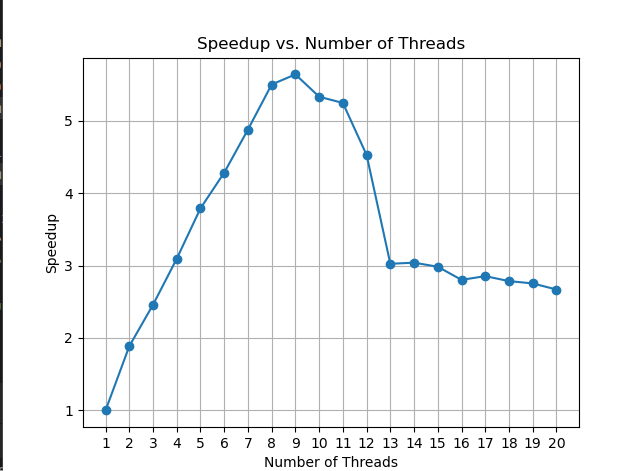
\includegraphics[width=\linewidth]{images/speedup.png}
  \caption{1907 Franklin Model D roadster. Photograph by Harris \&
    Ewing, Inc. [Public domain], via Wikimedia
    Commons. (\url{https://goo.gl/VLCRBB}).}
  \Description{A woman and a girl in white dresses sit in an open car.}
\end{figure}

Your figures should contain a caption which describes the figure to
the reader.
 It's important to highlight the \textbf{thread management}. Since we are working with images we will have to do some simples calculus to determine the amount of work that
 each thread will be given. For that we must perform two calculations (one for RGB and one for the grey scale). For the RGB  we will calculate $\texttt{WIDTH * HEIGHT * 3}$ and to obtain the \texttt{CHUNK\_SIZE\_RGB} we just divide $\texttt{WIDTH * HEIGHT * 3}$  by \texttt{N\_THREADS}. For the grey scale it's similar but we don't multiply by 3. Now we will have the work that will be balanced between threads.
  It's important to highlight the \textbf{thread management}. Since we are working with images we will have to do some simples calculus to determine the amount of work that
 each thread will be given. For that we must perform two calculations (one for RGB and one for the grey scale). For the RGB  we will calculate $\texttt{WIDTH * HEIGHT * 3}$ and to obtain the \texttt{CHUNK\_SIZE\_RGB} we just divide $\texttt{WIDTH * HEIGHT * 3}$  by \texttt{N\_THREADS}. For the grey scale it's similar but we don't multiply by 3. Now we will have the work that will be balanced between threads.
  It's important to highlight the \textbf{thread management}. Since we are working with images we will have to do some simples calculus to determine the amount of work that
 each thread will be given. For that we must perform two calculations (one for RGB and one for the grey scale). For the RGB  we will calculate $\texttt{WIDTH * HEIGHT * 3}$ and to obtain the \texttt{CHUNK\_SIZE\_RGB} we just divide $\texttt{WIDTH * HEIGHT * 3}$  by \texttt{N\_THREADS}. For the grey scale it's similar but we don't multiply by 3. Now we will have the work that will be balanced between threads.
  It's important to highlight the \textbf{thread management}. Since we are working with images we will have to do some simples calculus to determine the amount of work that
 each thread will be given. For that we must perform two calculations (one for RGB and one for the grey scale). For the RGB  we will calculate $\texttt{WIDTH * HEIGHT * 3}$ and to obtain the \texttt{CHUNK\_SIZE\_RGB} we just divide $\texttt{WIDTH * HEIGHT * 3}$  by \texttt{N\_THREADS}. For the grey scale it's similar but we don't multiply by 3. Now we will have the work that will be balanced between threads.
  It's important to highlight the \textbf{thread management}. Since we are working with images we will have to do some simples calculus to determine the amount of work that
 each thread will be given. For that we must perform two calculations (one for RGB and one for the grey scale). For the RGB  we will calculate $\texttt{WIDTH * HEIGHT * 3}$ and to obtain the \texttt{CHUNK\_SIZE\_RGB} we just divide $\texttt{WIDTH * HEIGHT * 3}$  by \texttt{N\_THREADS}. For the grey scale it's similar but we don't multiply by 3. Now we will have the work that will be balanced between threads.
  It's important to highlight the \textbf{thread management}. Since we are working with images we will have to do some simples calculus to determine the amount of work that
 each thread will be given. For that we must perform two calculations (one for RGB and one for the grey scale). For the RGB  we will calculate $\texttt{WIDTH * HEIGHT * 3}$ and to obtain the \texttt{CHUNK\_SIZE\_RGB} we just divide $\texttt{WIDTH * HEIGHT * 3}$  by \texttt{N\_THREADS}. For the grey scale it's similar but we don't multiply by 3. Now we will have the work that will be balanced between threads.

The ``\verb|figure|'' environment should be used for figures. One or
more images can be placed within a figure. If your figure contains
third-party material, you must clearly identify it as such, as shown
in the example below.
The ``\verb|figure|'' environment should be used for figures. One or
more images can be placed within a figure. If your figure contains
third-party material, you must clearly identify it as such, as shown
in the example below.
The ``\verb|figure|'' environment should be used for figures. One or
more images can be placed within a figure. If your figure contains
third-party material, you must clearly identify it as such, as shown
in the example below.
The ``\verb|figure|'' environment should be used for figures. One or
more images can be placed within a figure. If your figure contains
third-party material, you must clearly identify it as such, as shown
in the example below.
The ``\verb|figure|'' environment should be used for figures. One or
more images can be placed within a figure. If your figure contains
third-party material, you must clearly identify it as such, as shown
in the example below.
The ``\verb|figure|'' environment should be used for figures. One or
more images can be placed within a figure. If your figure contains
third-party material, you must clearly identify it as such, as shown
in the example below.
The ``\verb|figure|'' environment should be used for figures. One or
more images can be placed within a figure. If your figure contains
third-party material, you must clearly identify it as such, as shown
in the example below.
The ``\verb|figure|'' environment should be used for figures. One or
more images can be placed within a figure. If your figure contains
third-party material, you must clearly identify it as such, as shown
in the example below.

\subsection{\textbf{Q\&A}}
\texttt{TODO} Questions to ask the teacher.
\bibliographystyle{acm}
\bibliography{refs}

\end{document}